\documentclass[9pt]{beamer}

\usetheme[progressbar=frametitle]{metropolis}

\usepackage{appendixnumberbeamer}
\usepackage[spanish]{babel}
\usepackage[utf8x]{inputenc}
\usepackage{stmaryrd}
\usepackage{graphicx}
\def\Put(#1,#2)#3{\leavevmode\makebox(0,0){\put(#1,#2){#3}}}

\usepackage[spanish]{babelbib}
\usepackage{cmbright}                %font
\usepackage{url}
\usepackage{catchfilebetweentags}    %inclusión de pedazos de código
\usepackage{amsmath}
\usepackage{latex/agda}
\usepackage{unicode}
\usepackage{amssymb}
\usepackage{wasysym}

\newcommand{\sangrar}{\hspace{3ex}}
\newcommand{\saltar}{\vspace{1ex}}
\newcommand{\llenar}{\vskip0pt plus 1filll}

\title{construyendo tipos de datos con containers}
%\subtitle{y programando genéricamente}
\author{Eugenia Simich}
\date{20 de octubre de 2016}
\institute{\large XIV JCC}


\begin{document}
\maketitle

{
\usebackgroundtemplate{\includegraphics[height=\paperheight]{img/container3}}
\begin{frame}[plain]
\end{frame}
}

\begin{frame}[plain]
  $$S\ \triangleleft\ P = \Sigma [s \in S]\, P_s$$
\end{frame}


\begin{frame}{vistazo previo}
  \setbeamertemplate{section in toc}[sections numbered]
  \tableofcontents
\end{frame}

\begin{frame}{para comenzar...}
  \only<1>{
  esta charla se trata de
  \begin{itemize}
  \item \alert{programación genérica}
  \item en \alert{Agda} 
  \item (o en cualquier lenguaje con \alert{tipos dependientes})
  \end{itemize}}
  \only<2>{
  ¿y qué es...
  \begin{itemize}
  \item ... la \alert{programación genérica}?
  \item ... \alert{Agda}? 
  \item ... los \alert{tipos dependientes}?
  \end{itemize}}
\end{frame}

\section{motivaci\'on: programaci\'on gen\'erica}

\begin{frame}{algunos tipos de datos}
  \begin{block}{\framebox{booleanos}}
    \ExecuteMetaData[latex/Agda.tex]{bool}
  \end{block}
  \pause
  \begin{block}{\framebox{naturales}}
    \ExecuteMetaData[latex/Agda.tex]{nat}
  \end{block}
\end{frame}

\subsection{algunos programas gen\'ericos}
\begin{frame}[fragile]{algunos programas}
  \begin{itemize}
  \item programemos la función identidad...
    \pause
    \begin{columns}[T,onlytextwidth]
      \column{0.5\textwidth}
      \begin{block}{...de booleanos}
        \ExecuteMetaData[latex/Agda.tex]{idbool}
      \end{block}
      \pause
      \column{0.5\textwidth}
      \begin{block}{...y de naturales}
        \ExecuteMetaData[latex/Agda.tex]{idnat}
      \end{block}
      \pause
    \end{columns}
  \item ¿podremos construir una función identidad que {\it funcione} en ambos casos?\\ \saltar
    \pause
    ¡simple!\\
    \ExecuteMetaData[latex/Agda.tex]{id}
  \end{itemize}
\end{frame}

\begin{frame}{algunos programas}
  \begin{itemize}
  \item programemos ahora una función de comparación por igualdad...
    \pause
    \begin{columns}[T,onlytextwidth]
      \column{0.5\textwidth}
      \begin{block}{...para booleanos}
        \ExecuteMetaData[latex/Agda.tex]{eqbool}
      \end{block}
      \pause
      \column{0.5\textwidth}
      \begin{block}{...y para naturales}
        \ExecuteMetaData[latex/Agda.tex]{eqnat}
      \end{block}
      \pause
    \end{columns}
  \item ¿podremos construir una función de equivalencia \alert{genérica}?\\
    es decir, ¿podremos construir una función \AgdaFunction{eq} : $A \to A \to \AgdaDatatype{Bool}$?\\ \vspace{-0.3ex}
    {\hspace{5ex}\small (al menos para $A$ reemplazable por \AgdaDatatype{Bool}, \AgdaDatatype{Nat})}
    \pause
  \item ¿qué ganaríamos con hacerlo?
  \end{itemize}
\end{frame}


\subsection{universos}

\begin{frame}{programando gen\'ericamente}
  en Agda se puede, con un \emph{truco}: \alert{universos}
  \pause
  \begin{enumerate}
    \item comencemos definiendo un tipo \AgdaDatatype{Name}:\\ \saltar
      \ExecuteMetaData[latex/Agda.tex]{Name}
      \pause
    \item y una función:\\ \saltar
      \ExecuteMetaData[latex/Agda.tex]{Nameext}
      \pause
  \end{enumerate}
  \begin{itemize}
    \item ahora podemos definir: \\ \saltar
      \ExecuteMetaData[latex/Agda.tex]{eqt} \pause
      \hspace{5ex}\AgdaFunction{eq} \AgdaInductiveConstructor{nat}\hspace{0.9ex}   = \only<6>{\AgdaFunction{eqnat}}\\
      \hspace{5ex}\AgdaFunction{eq} \AgdaInductiveConstructor{bool} = \only<6>{\AgdaFunction{eqbool}}
  \end{itemize}
\end{frame}


{
\usebackgroundtemplate{\includegraphics[height=\paperheight,width=\paperwidth]{img/pipe}}
\begin{frame}[plain]
\end{frame}
}


\begin{frame}{receta para construir universos}
  \pause
  \begin{enumerate}
  \item definir un tipo de \emph{códigos sintácticos}, por ejemplo, \AgdaDatatype{U}:\\ \saltar
    \ExecuteMetaData[latex/U.tex]{U}
    \pause
  \item y una función de \emph{extensión}:\\ \saltar
    \ExecuteMetaData[latex/U.tex]{Uext}
    \pause
  \item descansar, acabamos de crear un universo
  \end{enumerate}
\end{frame}

\section{constructores de tipos}

\begin{frame}[fragile]{algunos constructores de tipos de datos}
    \begin{description}
    \item[\framebox{listas}]\ExecuteMetaData[latex/Agda.tex]{list}
      \pause
    \item[\framebox{maybe}]\ExecuteMetaData[latex/Agda.tex]{maybe}
      \pause
    \item[\framebox{árboles}]\ExecuteMetaData[latex/Agda.tex]{tree}
      \pause
    \item[\framebox{streams}]\ExecuteMetaData[latex/Agda.tex]{stream}
    \end{description}
    \Put(240,190){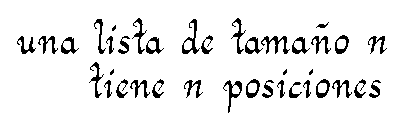
\includegraphics[height=4cm]{img/streams}}
\end{frame}

\begin{frame}{map}
  \begin{itemize}
  \item programemos funciones de mapeo...
    \begin{block}{...para listas}\ExecuteMetaData[latex/Agda.tex]{maplist}\end{block}
    \vspace{1cm}
    \begin{center}\hspace{-2cm}\includegraphics[scale=0.5]{img/maplist}\end{center}
  \end{itemize}
\end{frame}

\begin{frame}{map}
  \begin{itemize}
  \item programemos funciones de mapeo...
    \begin{block}{...para árboles}\ExecuteMetaData[latex/Agda.tex]{maptree}\end{block}
    \vspace{1cm}
    \begin{center}\includegraphics[scale=0.5]{img/maptree}\end{center}
  \end{itemize}
\end{frame}

\begin{frame}{map}
  \begin{itemize}
  \item programemos funciones de mapeo...
    \begin{block}{...para streams}\ExecuteMetaData[latex/Agda.tex]{mapstream}\end{block}
    \vspace{1.2cm}
    \begin{center}\hspace{-2cm}\includegraphics[scale=0.5]{img/mapstream}\end{center}
  \end{itemize}
\end{frame}


\begin{frame}{map}
  \begin{itemize}
  \item programemos funciones de mapeo...
    \begin{block}{...para maybe}\ExecuteMetaData[latex/Agda.tex]{mapmaybe}\end{block}
    \vspace{1.2cm}
    \begin{center}\hspace{-2cm}\includegraphics[scale=0.5]{img/mapmaybe}\end{center}
  \end{itemize}
\end{frame}

\subsection{funtores}

\begin{frame}{funtores = constructores mapeables}
  \begin{itemize}
  \item las listas, los árboles, los streams, entre otros constructores de tipos son \alert{mapeables}
  \item llamaremos \alert{funtores} a estos constructores\\ {\small(deberán preservar identidades y composiciones)} 
  \item ¿podremos construir una \AgdaFunction{map} genérica?
  \end{itemize}
\end{frame}


\section{containers}

\begin{frame}{containers}
  \fbox{\begin{minipage}{4 in} los \alert{containers} son una representación alternativa de ciertos tipos de datos\end{minipage}}
  \begin{itemize}
  \item[]¿qué tipos de datos?
  \item[]aquellos que \emph{contienen} otros datos
  \item[] y pueden pensarse como \alert{formas con posiciones}
  \end{itemize}
  \vspace{2cm}
  \begin{flushright}veamos algunos ejemplos...\end{flushright}
\end{frame}


\begin{frame}{ejemplo: listas}
  \begin{itemize}
  \item las listas tienen las siguientes formas:\saltar
    \begin{center}\hspace{-2cm}\includegraphics[scale=0.5]{img/elistsh.eps}\end{center}
    \pause
    \begin{flushright}\hspace{-2cm}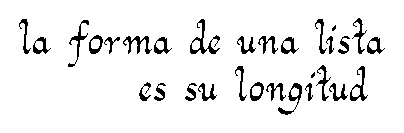
\includegraphics[scale=0.5]{img/laformadeunalistaessulongitud.eps}\end{flushright}
    \pause
  \item y cada forma tiene un conjunto de posiciones a ser llenadas con datos:\saltar
    \begin{center}\hspace{-2cm}\includegraphics[scale=0.5]{img/elistpos.eps}\end{center}
    \pause
    \begin{flushright}\hspace{-2cm}\includegraphics[scale=0.5]{img/unalistadetamanontienenposiciones.eps}\end{flushright}
    \pause
  \end{itemize}
  \begin{itemize} \setbeamertemplate{itemize item}[triangle]
  \item el tipo \AgdaDatatype{Nat} representa de forma unívoca a las formas de listas
  \item dada una forma $n$ (una longitud $n$), el conjunto de posiciones es $\{ 0, \ldots, n-1\}$
  \end{itemize}
\end{frame}

\begin{frame}{ejemplo: streams}
  \begin{itemize}
  \item todos los streams tienen la misma forma:\saltar
    \begin{center}\hspace{-2cm}\includegraphics[scale=0.5]{img/estreamsh.eps}\end{center}
    \pause
  \item y $\aleph_0$ posiciones a ser llenadas con datos: \saltar
    \begin{center}\hspace{-2cm}\includegraphics[scale=0.5]{img/estreampos.eps}\end{center}
    \pause
  \end{itemize}
  \begin{itemize} \setbeamertemplate{itemize item}[triangle]
  \item el tipo \AgdaDatatype{Unit} (con un único habitante) representa el conjunto de formas de streams:\\
      \ExecuteMetaData[latex/Agda.tex]{top}
  \item el conjunto de posiciones es \AgdaDatatype{Nat}\\\vspace{-0.5ex} {\small (para toda forma)}
  \end{itemize}
\end{frame}

\begin{frame}{ejemplo: maybe}
  \begin{itemize}
  \item un habitante de maybe puede tener dos formas: \saltar
    \begin{center}\hspace{-2cm}\includegraphics[scale=0.5]{img/emaybe.eps}\end{center}
    \pause
  \item la forma ``nothing'' no tiene posiciones
  \item la forma ``just'' tiene una posición
    \pause
  \end{itemize}
  \begin{itemize} \setbeamertemplate{itemize item}[triangle]
  \item el tipo \AgdaDatatype{Bool} (con dos habitantes) puede representar al conjunto de formas del container maybe
  \item los tipos \AgdaDatatype{$\emptyset$} (conjunto vacío) y \AgdaDatatype{Unit} representan las posiciones, para cada forma
  \end{itemize}
\end{frame}


\begin{frame}{containers}
  \begin{itemize}
  \item representación alternativa de (algunos) constructores de tipos (como las listas, los árboles, etc)
  \item segrega \alert{estructura} de \alert{contenido}
  \item las listas, los árboles, los streams, pueden ser vistos como \alert{contenedores} de otros datos
  \end{itemize}
  \pause
  \metroset{block=fill}
  \begin{block}{definición}
    un \alert{container} es un conjunto de formas, y por cada forma un conjunto de posiciones\\ \saltar
    si $S$ es un conjunto de formas y $P_x$ el conjunto de posiciones dentro de la forma $x \in S$:\\
    $$S \ \AgdaInductiveConstructor{$\triangleleft$}\ P$$
    es un container\saltar
  \end{block}
\end{frame}


\begin{frame}{retomando los ejemplos}
  \begin{itemize}
  \item[] un container es un par $S \ \AgdaInductiveConstructor{$\triangleleft$}\ P$ donde
    \begin{itemize}
      \item $S$ es un conjunto de formas
      \item $P_s$ es una familia de conjuntos de posiciones (un conjunto por cada forma)
    \end{itemize}
  \end{itemize}
  \only<1>{\vspace{8cm}}
  \pause
  \begin{columns}[T,onlytextwidth]
    \column{0.7\textwidth}
    \metroset{block=fill}
    \only<2->{\begin{exampleblock}{listas}\ExecuteMetaData[latex/Container.tex]{clist}\end{exampleblock}}
    \only<2>{\vspace{8cm}}
    \only<3->{\begin{exampleblock}{stream}\ExecuteMetaData[latex/Container.tex]{cstream}\end{exampleblock}}
      \only<3>{\vspace{4cm}}
    \only<4->{\begin{exampleblock}{maybe}\ExecuteMetaData[latex/Container.tex]{cmaybe}\end{exampleblock}}
    \column{0.3\textwidth}
    \only<2->{\Put(10,-80){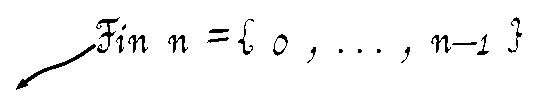
\includegraphics[width=\linewidth]{img/fin}}}
  \end{columns}
\end{frame}

\begin{frame}{llenando containers}
  \begin{itemize}
  \item los containers representan la \alert{estructura} de los tipos de datos\\ ¿cómo hacer para llenar la estructura con contenido? \\
    \pause
    \alert{asignando valores a las posiciones}\pause
  \item tomemos por ejemplo la lista $[\blacksquare, \newmoon, \blacklozenge]$ de tipo $X$\\ \saltar\saltar
    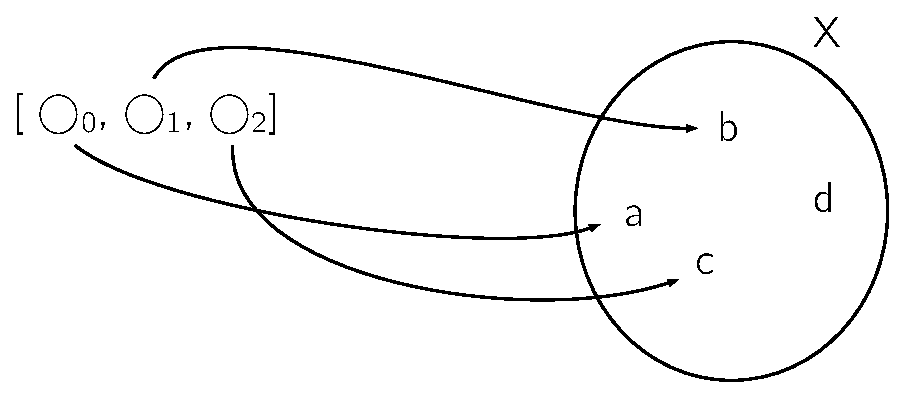
\includegraphics[scale=0.5]{img/listext.eps}
  \end{itemize}
\end{frame}

\begin{frame}{extensión de containers}
  los containers son un universo para representar constructores de tipos de datos, su \emph{extensión} le dará el significado original\\\saltar
  la extensión \alert{llena} el container\pause
    \metroset{block=fill}
    \begin{block}{definición}Dado un container $S\ \AgdaInductiveConstructor{$\triangleleft$ } P$ su \alert{extensión}
      $\llbracket S\ \AgdaInductiveConstructor{$\triangleleft$ } P \rrbracket $ es
      \begin{itemize}
      \item el conjunto de formas $S$
      \item por cada forma de $S$, una función de posiciones en valores
      \end{itemize}
      \end{block}
    \begin{exampleblock}{extensión de containers}
      \ExecuteMetaData[latex/Container.tex]{ext}
    \end{exampleblock}
    \begin{center}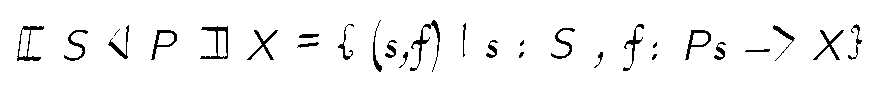
\includegraphics[scale=0.5]{img/ext.eps}
    \end{center}
\end{frame}

\begin{frame}{volviendo a las listas originales}
  \begin{itemize}
    \item la función de extensión reconstruye el tipo original
      $$\AgdaFunction{$\llbracket$ } \AgdaFunction{cList } \AgdaFunction{ $\rrbracket$} \cong \AgdaDatatype{List}$$
      \pause
    \item ejemplo: la lista $[\, \blacksquare,\, \newmoon,\, \newmoon\, ]$ de símbolos se representa:\\\saltar
      \ExecuteMetaData[latex/Container.tex]{l}
  \end{itemize}
  \llenar
\end{frame}


\begin{frame}{volviendo a las listas originales}
    \begin{itemize}
    \item la función de extensión reconstruye el tipo original
      $$\AgdaFunction{$\llbracket$ } \AgdaFunction{cList } \AgdaFunction{ $\rrbracket$} \cong \AgdaDatatype{List}$$
    \item  o mejor, reconstruimos las funciones:\\ \saltar
      \ExecuteMetaData[latex/Container.tex]{listconstructors}
      \Put(115,135){
\includegraphics[scale=0.4]{img/empty2}}
      \pause
    \item así la lista $[\, \blacksquare,\, \newmoon,\, \newmoon\, ]$ es simplemente:\\\saltar
      \ExecuteMetaData[latex/Container.tex]{lprime}
    \end{itemize}
    \llenar
\end{frame}


\begin{frame}{más ejemplos}
  algunos containers triviales
  \begin{itemize}
  \item el container identidad representa al funtor identidad:\\\saltar
    \begin{columns}[T,onlytextwidth]
      \onslide<2->{ \column{0.6\textwidth} \ExecuteMetaData[latex/Container.tex]{cId}}
      \onslide<1->{ \column{0.4\textwidth} \includegraphics[scale=0.45]{img/cid}}
    \end{columns}
    \onslide<3->{ entonces\\ \hspace{15ex}$\AgdaFunction{$\llbracket$ } \AgdaFunction{cId } \AgdaFunction{ $\rrbracket$}\ X \cong X$}
  \onslide<4->{\item el container constante ignora el argumento y siempre construye un tipo constante:\\}
    \begin{columns}[T,onlytextwidth]
      \onslide<5->{ \column{0.6\textwidth} \ExecuteMetaData[latex/Container.tex]{cK}}
      \onslide<4->{ \column{0.4\textwidth} \includegraphics[scale=0.45]{img/ck}}
    \end{columns}
    \onslide<6->{ entonces\\ \hspace{15ex}$\AgdaFunction{$\llbracket$ } \AgdaFunction{cK}\ A\ \AgdaFunction{ $\rrbracket$}\ X \cong A$}
  \end{itemize}
\end{frame}


\begin{frame}{map de containers}
  \begin{itemize}
  \item si $C$ es un container, \AgdaFunction{$\llbracket$} $C$ \AgdaFunction{$\rrbracket$} : \AgdaDatatype{Set} $\to$ \AgdaDatatype{Set}
  \item \AgdaFunction{$\llbracket$} $C$ \AgdaFunction{$\rrbracket$} es nuevamente un constructor de tipos..
  \item ...pero, ¿es funtorial? ¿podremos construir una función \AgdaFunction{map} de containers?
    \pause
  \item en el caso de las listas, por ejemplo:
  \end{itemize} 
  \includegraphics[scale=0.4]{img/map.eps}\\\saltar
  
  transformamos la lista $[x_1,x_2,x_3]$ en la lista $[y_4,y_1,y_3]$ simplemente \emph{componiendo} las funciones
\end{frame}

\begin{frame}{map de containers}
  \metroset{block=fill}
  \llenar
  \begin{exampleblock}{map}
    \ExecuteMetaData[latex/Container.tex]{map}
  \end{exampleblock}
  \llenar
  \pause
  ¡funciona para todo container! ¡obtuvimos nuestra \AgdaFunction{map} genérica!
\end{frame}

\begin{frame}{construcciones con containers}
  podemos construir también:
  \begin{itemize}
    \item producto de containers
    \item suma de containers (Either de Haskell)
    \item exponencial de containers (funciones desde una constante) 
    \item composición (para obtener listas de árboles, árboles de streams, etc)
  \end{itemize}
\end{frame}

\section{morfismos de containers}
\begin{frame}[fragile]{morfismos de containers}
  \fbox{\begin{minipage}{4 in} containers = esqueletos \hspace{1cm} morfismos = funciones entre esqueletos\end{minipage}}
  \vspace{3ex}
    \begin{itemize}
    \item Hay funciones que \emph{hacen cosas con la estructura sin tocar el contenido} (\alert{sólo lo reubican})
      \begin{itemize}
      \item decapitar listas
      \item aplanar árboles
      \item obtener subconjuntos finitos de un stream
      \end{itemize}\saltar
  \item ¿podremos construir un universo para representar estas funciones?
  \end{itemize}
\end{frame}

\begin{frame}[fragile]{ejemplo: cabeza de lista}
  ¿cómo la expresamos la función \AgdaFunction{head} de listas en términos de funciones entre los containers \AgdaFunction{cList} y \AgdaFunction{cMaybe}?\\
  \pause
  recordemos:
  \begin{columns}[T,onlytextwidth]
    \column{0.4\textwidth}
    \hspace{-1ex}\ExecuteMetaData[latex/Container.tex]{clist}
    \column{0.6\textwidth}
    \ExecuteMetaData[latex/Container.tex]{cmaybe}
  \end{columns}
  \pause
  la función \AgdaFunction{head} transforma un \AgdaFunction{cList} en un \AgdaFunction{cMaybe}.\\\saltar
  \begin{center}\includegraphics[scale=0.4]{img/head.eps}\end{center}
  en resumen,
    \begin{itemize}
    \item la forma \AgdaInductiveConstructor{zero} se transforma en \AgdaInductiveConstructor{false}
    \item la forma \AgdaInductiveConstructor{suc} $n$ se transforma en \AgdaInductiveConstructor{true}
    \item lo que guarda la única posición de la forma \AgdaInductiveConstructor{true} proviene de la \emph{primera} posición de la lista
    \end{itemize}
\end{frame}


\begin{frame}{morfismos de containers}
  \metroset{block=fill}
  \begin{block}{definición}
    un \alert{morfismo de container} entre los containers $(S_1\, \AgdaInductiveConstructor{$\triangleleft$}\, P_1)$ y $(S_2\, \AgdaInductiveConstructor{$\triangleleft$}\, P_2)$ es un par de funciones $(f_s, f_p)$ donde:
    \begin{itemize}
    \item $f_s\ :\ S_1 \to S_2\quad$ transforma las formas
    \item $f_p\ :\ (x\, :\, S_1) \to P_2\, (f_s\, x) \to P_1\, x\quad$ reubica las posiciones
    \end{itemize}\saltar
  \end{block}
  notamos $C\, \AgdaFunction{$\Rightarrow$}\, D$ a los morfismos entre los containers $C$ y $D$.
\end{frame}

\begin{frame}{ejemplo: cabeza de lista (continuación)}
  \metroset{block=fill}
  para concluir con el ejemplo
  \begin{exampleblock}{chead}
    \ExecuteMetaData[latex/Container.tex]{chead}
  \end{exampleblock}
  \pause
  también podemos \emph{llenar} los esqueletos de funciones, con la extensión de morfismos \AgdaFunction{$\llbracket$} $\_$ \AgdaFunction{$\rrbracket_{m}$}\\ \saltar
  \begin{exampleblock}{head}
  \ExecuteMetaData[latex/Container.tex]{head}
  \end{exampleblock}
\end{frame}

\begin{frame}{comentarios al margen}
  punto de vista categórico: los containers y sus morfismos forman una categoría
  \begin{itemize}
  \item la categoría es bicartesiana cerrada (cuenta con productos, coproductos, exponenciales, inicial y terminal)
  \item la extensión de un container es un endofuntor en Set
  \item la extensión de los morfismos, las transformaciones naturales\\ ({\small \emph{todas y sólo todas las transf. naturales}})  
  \end{itemize}
\end{frame}

\begin{frame}{conclusiones y extensiones}
  hemos introducido a los containers y algunas propiedades:
  \begin{itemize}
  \item forma alternativa de representación de (ciertos) tipos de datos
  \item universo de constructores de tipos
  \item útiles para la programación genérica
  \item morfismos de containers como funciones entre esqueletos
  \end{itemize}
  además se puede ver que es posible
  \begin{itemize}
  \item representar funtores polinomiales
  \item representar tipos estrictamente positivos (útiles en la programación total, i.e. garantizando terminación)
  \end{itemize}
  algunas extensiones posibles son:
  \begin{itemize}
  \item representar funtores de más de un argumento
  \item representar funtores indexados (para construir tipos dependientes)
  \end{itemize}
\end{frame}


\appendix

\begin{frame}[standout]
  \llenar
  
  ¡gracias!
  ¿preguntas?

  \llenar

  pueden encontrar este (y más) material en \url{https://www.github.com/eugeniasimich/containers}

\end{frame}

\begin{frame}{referencias}
  \setbeamertemplate{bibliography item}[triangle]
  \nocite{*}
  \bibliography{jcc}
  \bibliographystyle{abbrv}

\end{frame}

%% \begin{frame}[standout]
%% pueden encontrar este (y más) material en \url{https://www.github.com/eugeniasimich/containers}
%% \end{frame}


\end{document}




\section{funtores polinomiales}

\begin{frame}{¿qué es un polinomio?}
 \begin{itemize}
 \item en el sentido más básico, un polinomio es una función $p : \mathbb{N} \to \mathbb{N}$ de la forma: $$p(x) = \sum_{n \in \mathbb{N}} a_{n} \, x^{n}$$
 \item pueden definirse por inducción como:
   \begin{itemize}
   \item la función identidad es un polinomio
   \item las constantes son polinomios
   \item si $p$ y $q$ son polinomios entonces $p \times q$ es un polinomio, dado por $$(p \times q) (x) = p(x) \times q(x)$$
   \item si $p$ y $q$ son polinomios entonces $p + q$ es un polinomio, dado por $(p + q) (x) = p(x) + q(x)$
   \end{itemize}
 \end{itemize}
\end{frame}

\begin{frame}{¿qué es un \alert{funtor} polinomial?}
 \begin{itemize}
% \item un funtor polinomial es un funtor $P : \AgdaDatatype{Set} \to \AgdaDatatype{Set}$ de la forma: $$P\ X = \sum_{b \in B} \, X^{E_b}$$
 \item pueden definirse por inducción como:
   \begin{itemize}
   \item el funtor identidad \emph{Id} es un polinomial
   \item el funtor constante $K_{A}$ es polinomial, para todo $A : \AgdaDatatype{Set}$
   \item si $P$ y $Q$ son funtores polinomiales entonces $P\!\times\!Q$ es un funtor polinomial, dado por $$P\!\times\!Q\ X = P\ X \times Q\ X$$ $$\AgdaFunction{map}\, f\, (x,y) = (\AgdaFunction{map}_{P} f\, x, \AgdaFunction{map}_{Q} f\, y)$$
   \item si $P$ y $Q$ son funtores polinomiales entonces $P\!+\!Q$ es un funtor polinomial, dado por $$P\!+\!Q\ X = P\ X \uplus Q\ X$$ $$\AgdaFunction{map}\, f\, (\AgdaInductiveConstructor{left}\, x) = \AgdaFunction{map}_{P} f\, x $$
$$\AgdaFunction{map}\, f\, (\AgdaInductiveConstructor{right}\, y) = \AgdaFunction{map}_{Q} f\, y $$
   \end{itemize}
 \end{itemize}
\end{frame}

\begin{frame}{algunos funtores polinomiales}
  sea por ejemplo el funtor polinomial $M$:
  $$M\, X = \AgdaFunction{Unit} \uplus X$$
  es decir, 
  $$M = K_{\AgdaFunction{Unit}} + \mathit{Id} $$
  ¿a qué se parece? $M\, X$ tiene un elemento más que $X$
  $$\AgdaDatatype{Maybe}\, X = \AgdaInductiveConstructor{nothing}\ |\ \AgdaInductiveConstructor{just } X$$
  $$\mbox{¡ }M\, \cong\, \AgdaDatatype{Maybe}\mbox{ !}$$
\end{frame}

\begin{frame}{algunos funtores polinomiales}
  consideremos ahora el funtor polinomial $P$:
  $$P = \mathit{Id} \times \mathit{Id} $$
  aplicado a un tipo $X$ cualquiera:
  $$P\, X = X \times X$$
  ¿a qué se parece? 
  $$\AgdaDatatype{Pair}\, X = (\, X, X\, )$$
  $$\mbox{¡ }P\, \cong\, \AgdaDatatype{Pair}\mbox{ !}$$
\end{frame}

\begin{frame}{algunos funtores polinomiales}
  pero... ¿y si quisiera construir árboles, por ejemplo?
  $$\AgdaDatatype{Tree}\, X = \AgdaInductiveConstructor{leaf}\ X\ |\ \AgdaInductiveConstructor{node}\ (\AgdaDatatype{Tree}\, X, \AgdaDatatype{Tree}\, X\, )$$
  es decir que quisiéramos un funtor
  $$T\, X = X \uplus T\, X \times T\, X $$
  ¡pero no tenemos recursividad!
\end{frame}





\begin{frame}{¿para qué todo esto?}
\end{frame}

\section{containers como funtores polinomiales}

\begin{frame}{producto de containers}
  
\end{frame}

\begin{frame}{suma de containers}
  
\end{frame}

\begin{frame}{exponencial de containers}
  
\end{frame}

\begin{frame}{punto fijo}
  
\end{frame}


\begin{frame}{ejemplo: árboles binarios (toma dos)}
  
\end{frame}

